\documentclass[12pt,a4paper]{article}
%\documentclass[sansserif,12pt,a4paper]{article}

% example using pdftk to extract pages from a pdf file
% pdftk wpg_bounds.pdf cat 15 output output.pdf

\newcommand{\mbm}[1]{\mbox{\boldmath $#1$}}

\usepackage{graphicx,color,psfrag}

\usepackage{tabularx,colortbl}

\usepackage{amssymb}
\usepackage{amsfonts}
\usepackage{epsfig}

\usepackage[sans]{dsfont} % double stroke fonts
\usepackage{bbm} % bbm fonts

\usepackage{amsmath,bm}    % need for subequations

\newenvironment{rcase}
{\left. \begin{aligned}}
{\end{aligned}\right\rbrace}

%\usepackage{graphicx}   % need for figures
\usepackage{verbatim}   % useful for program listings
\usepackage{color}      % use if color is used in text
\usepackage{subfigure}  % use for side-by-side figures
\usepackage{hyperref}   % use for hypertext links, including those to external documents and URLs

\usepackage{scalefnt}
%\usepackage{txfonts}

\usepackage{theorem}

% this appears to preserve the original font in the theorems
\theorembodyfont{\upshape}

\theoremstyle{break}

\usepackage[top=2cm, bottom=2cm, left=2cm, right=2cm]{geometry}

\newcommand{\norm}[1]{\lVert#1\rVert}

%COLORS
\definecolor{gray}{rgb}{0.8,0.8,0.8}\newcommand{\gray}{\color{gray}}
\definecolor{darkgray}{rgb}{0.6,0.6,0.6}\newcommand{\darkgray}{\color{darkgray}}
\definecolor{white}{rgb}{1.0,1.0,1.0}\newcommand{\white}{\color{white}}

% gray box
\newcommand{\gbox}[1]{
  \begin{center}
    \fcolorbox{black}{gray}{
      \begin{minipage}[b]{0.98\textwidth}
        \begin{center}
          %\vspace{2mm}
          \begin{minipage}{0.97\textwidth}
            #1 
          \end{minipage}
          \vspace{2mm}
        \end{center}
      \end{minipage}
    }
  \end{center}
}

\newcommand{\wbox}[1]{
  \begin{center}
    \fcolorbox{black}{white}{
      \begin{minipage}[b]{0.98\textwidth}
        \begin{center}
          %\vspace{2mm}
          \begin{minipage}{0.97\textwidth}
            #1 
          \end{minipage}
          \vspace{2mm}
        \end{center}
      \end{minipage}
    }
  \end{center}
}

\begin{document}

\begin{figure}[t]
  \begin{center}
    \includegraphics[height=10cm]{xy_old.eps}
    \caption{Old $xy$}
    \label{fig:xy_old}
  \end{center}
\end{figure}

\begin{figure}[t]
  \begin{center}
    \includegraphics[height=10cm]{xy_new.eps}
    \caption{New $xy$}
    \label{fig:xy_new}
  \end{center}
\end{figure}

% ---------------------------------------------

\begin{figure}[t]
  \begin{center}
    \includegraphics[height=11cm]{phi_old.eps}
    \caption{Old $\phi$}
    \label{fig:phi_old}
  \end{center}
\end{figure}

\begin{figure}[t]
  \begin{center}
    \includegraphics[height=11cm]{phi_new.eps}
    \caption{New $\phi$}
    \label{fig:phi_new}
  \end{center}
\end{figure}


\end{document}

